\chapter{Evaluation}
% TODO: Compare results to those of more complex models; look at other papers
% and use their parameters
As mentioned in Chapter \ref{applications}, most of the practical applications
of metamaterials and photonic crystals come from their ability to control the
propagation of acoustic or electromagnetic waves. As such, it is important to
evaluate our model in terms of whether the results can translate to other
complex models.

To evaluate the performance and accuracy of our mass-spring model, we will
therefore compare our results to those produced in other papers, some with the
mass-spring model and some with more complex continuous models.

\section{Further work}
% TODO: Can split into what we can do in terms of different perturbations/
% grading etc; but also look at computing side, e.g. split into classes so
% easier to run simulations and get dispersion curves etc
% - compare the two different kind of perturbations. Is there a difference?
% Alternating mass one seems to be better. Amplitude is higher
There are many things that we can improve on and continue investigating for the
future. 

In terms of investigating deeper the challenges that might be faced when going
from simulations to a real world product, the following could be useful:
\begin{itemize}
\item Evaluating the robustness of our system to imperfections in the lattice.
This is crucial as real production systems have certain tolerances and are not
perfect. As such, it is important to be able to test how little changes in the
lattice can affect the edge states that we get, in terms of the strength of the
energy which is transmitted as well as the amount of energy which is dissipated
throughout the lattice.

\item Testing how small each layer of material can be to get a \textit{good
enough} edge state. So far in our discussions of the strips of cells, we have
been using strips with a large number of cells (e.g. $2N=40$) because we know
that the edge states decay exponentially outwards from the boundary, but this
may not be possible or cost effective when developing real products. Therefore,
it is important to study how the number of cells translates to the amount of
energy lost and how this might lead to unwanted energy elsewhere in the system
or interference with our edge state along the boundary. An example can be seen
in Figure~\ref{fig:smallvsbig}.
\end{itemize}

\begin{figure}
\centering
\begin{subfigure}[b]{.5\textwidth}
  \centering
  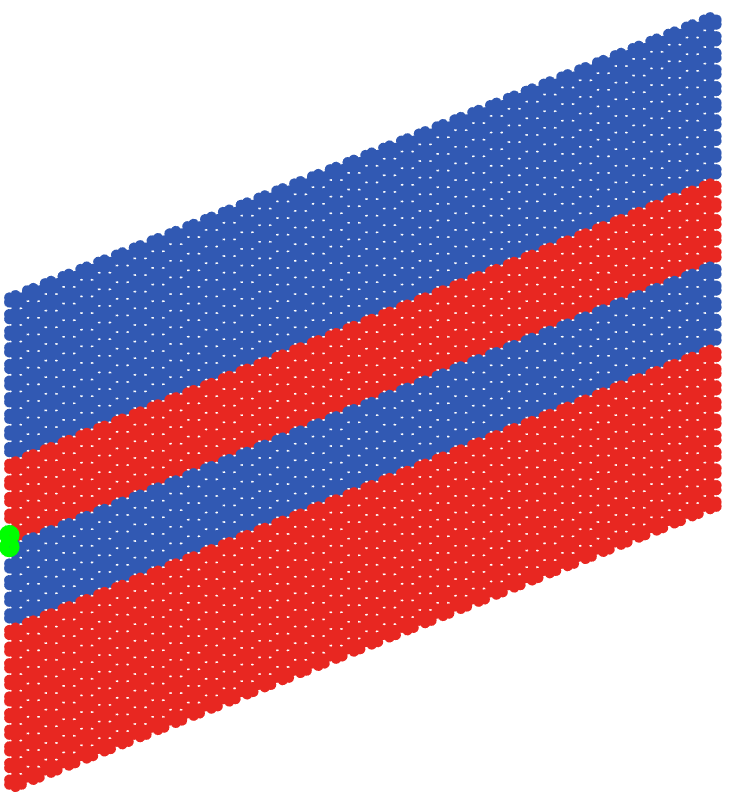
\includegraphics[width=0.7\linewidth]{imgs/svbthickarr.png}
  \caption{Arrangement of cells with $2N=10$.}
  \label{fig:sub1}
\end{subfigure}%
\begin{subfigure}[b]{.5\textwidth}
  \centering
  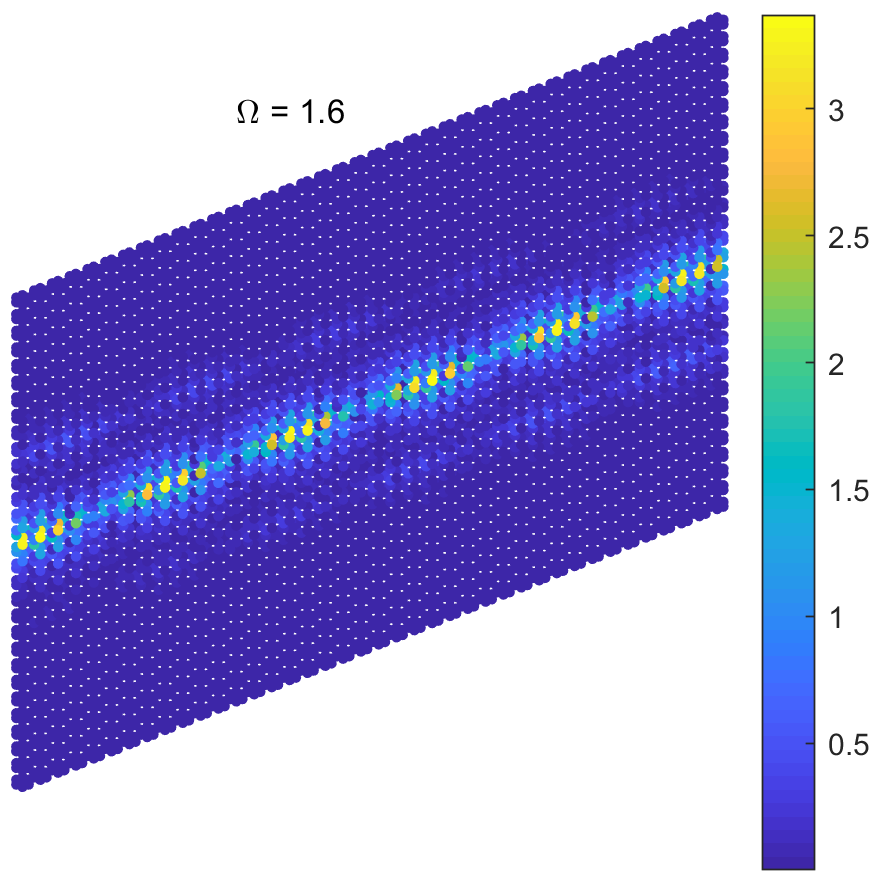
\includegraphics[width=0.9\linewidth]{imgs/svbthickscat.png}
  \caption{The plot of $|y_i|$ for each mass in each cell.}
  \label{fig:sub2}
\end{subfigure}

\medskip
\begin{subfigure}[b]{.5\textwidth}
  \centering
  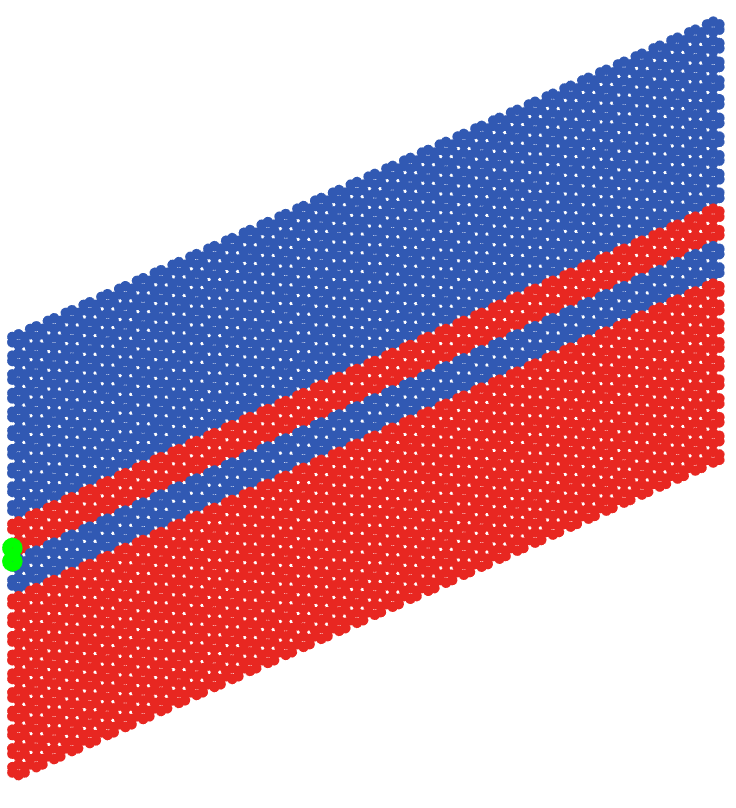
\includegraphics[width=0.7\linewidth]{imgs/svbthinarr.png}
  \caption{Arrangement of cells with $2N=4$.}
  \label{fig:sub1}
\end{subfigure}%
\begin{subfigure}[b]{.5\textwidth}
  \centering
  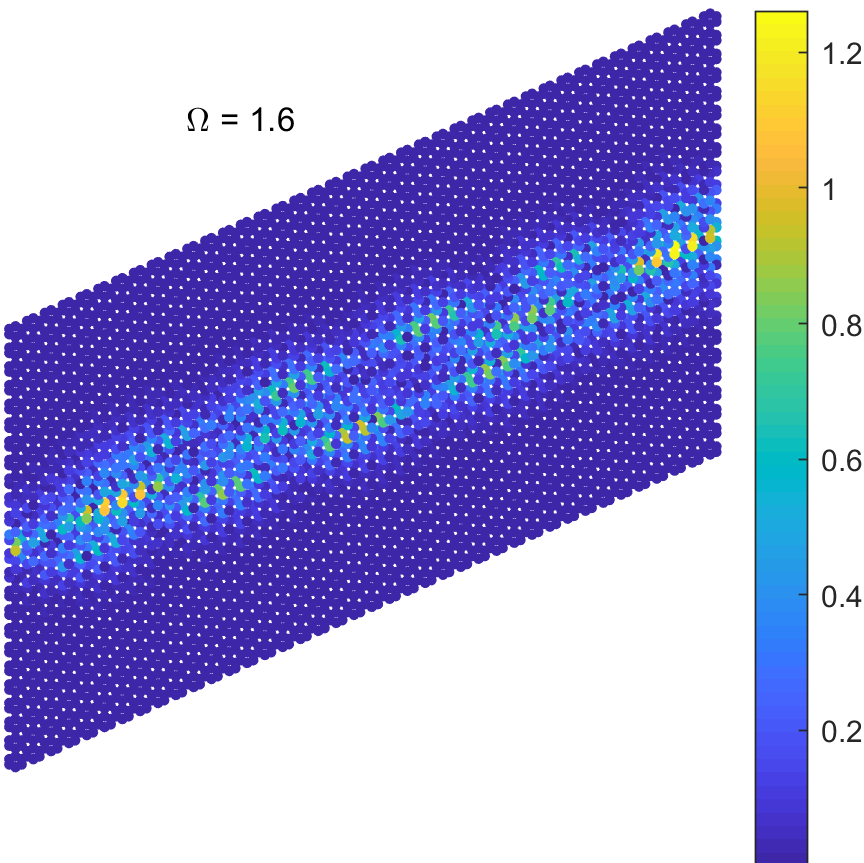
\includegraphics[width=0.9\linewidth]{imgs/svbthinscat.png}
  \caption{The plot of $|y_i|$ for each mass in each cell.}
  \label{fig:sub2}
\end{subfigure}

\medskip
\begin{subfigure}[b]{.5\textwidth}
  \centering
  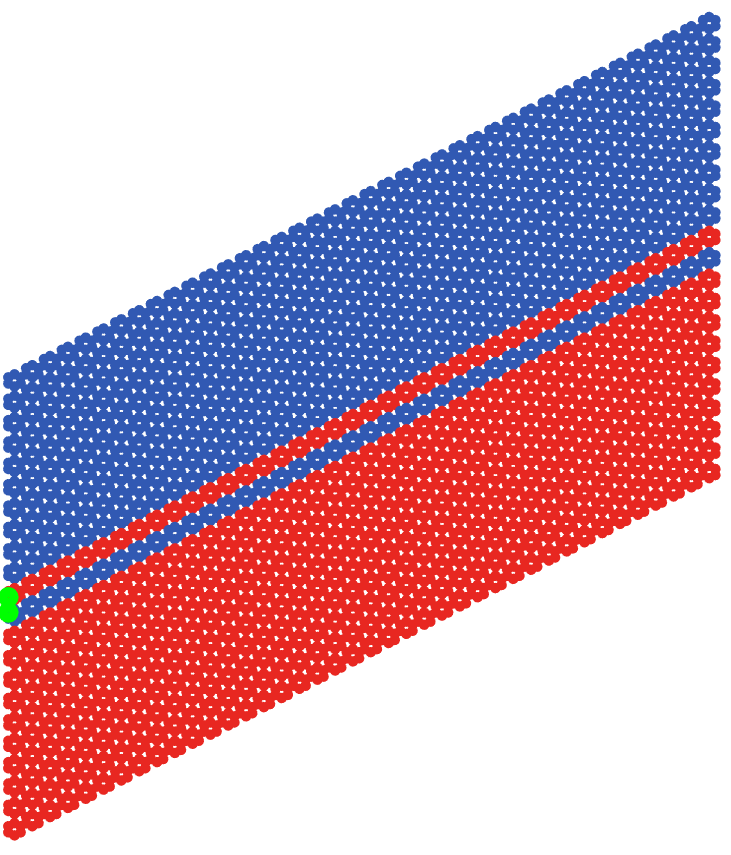
\includegraphics[width=0.7\linewidth]{imgs/svbthinnerarr.png}
  \caption{Arrangement of cells with $2N=2$.}
  \label{fig:sub1}
\end{subfigure}%
\begin{subfigure}[b]{.5\textwidth}
  \centering
  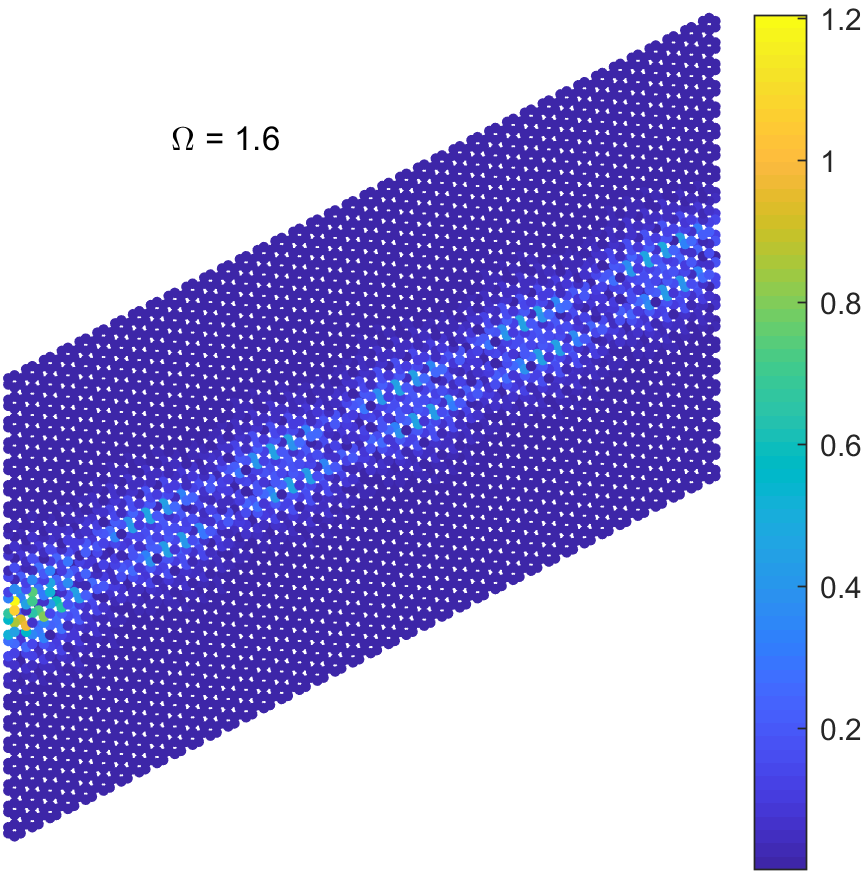
\includegraphics[width=0.9\linewidth]{imgs/svbthinnerscat.png}
  \caption{The plot of $|y_i|$ for each mass in each cell.}
  \label{fig:sub2}
\end{subfigure}
\caption{Scattering simulation to show the differences in amplitude and
  dissipation of energy for hexagonal boundaries of different thicknesses using
  the cells as defined in Figure~\ref{fig:hexstripMrotated}.}
\label{fig:smallvsbig}
\end{figure}

In terms of improving the workflow for the generation of these results for
other geometries and topologies, we could implement the following:
\begin{itemize}
\item Move to an object-oriented programming model. We can implement the
concepts of shapes and topologies as interfaces which contain information about
the required geometries. Then we can create specific classes corresponding to
actual shapes to extend those interfaces. We can then have our core code which
generates the dispersion relations and scattering simulations work based on the
interface implemented, rather than being specific to one shape class. This
should be relatively straightforward to implement, as most of the code to solve
for dispersion curves and scattering simulations is the same for any shape. The
only big difference for different topologies is the formation of the
eigen-problem matrix, which is a really mechanical but time-consuming
procedure, and so this will make testing out new shapes or different connection
of masses much easier.

\item To take the above idea and make it even more user-friendly, we could
create a graphical user interface where a user can choose things like the shape
of the cell, the position of masses within the cell and how the masses are
connected. This would allow faster and simpler prototyping of new designs.
\end{itemize}
